\documentclass{article}
\title{Prelim Outline}
\author{Shivesh Pathak}
\usepackage[margin=1.0in]{geometry}
\usepackage{graphicx}
\usepackage{float}
\begin{document}

\section{Introduction and methods}
\textit{The goal of the introduction is to show the reader that the project is valuable. Should be x pages, other 5-x page will be methods.}

\paragraph{Overall goal}
We want to understand the low energy behavior of the cuprate superconductors.
\\
\textit{This paragraph will be outlining the various phenomenon attributed with the cuprates, e.g. the many phases.}

\paragraph{Barrier to achieving goal}
The strong coupling between magnetic, charge, and lattice degrees of freedom in the cuprates makes writing down an accurate low energy effective theory very challenging.
\\
\textit{This paragraph will outline the many experiments that show the strong coupling between these many degrees of freedom.}

\paragraph{Current state of the art}
Many theoretical approaches to generating a low energy model for the cuprates have been attempted with varying degrees of success.
\\
\textit{This paragraph will outline the various approaches people have tried to generate effective theories. Hole doped, electron doped, pen and paper, computational, energetics, one- and two-body properties.}

\paragraph{Advancement to the state of the art}
We propose that a density matrix downfolding approach using \textit{ab initio} quantum Monte Carlo calculations can generate an effective model which can accurately describe low-energy properties and energetics for the infinite layer electron-doped cuprates at zero temperature and dopings of x=0, 0.125, 0.25.
\\
\textit{This paragraph will describe in detail each of the conditions in the thesis sentence.}

\paragraph{Density matrix down folding} 
The density matrix downfolding method allows us to downfold a first-principles Hamiltonian into a low-energy effective theory by mapping the downfolding problem to a linear regression problem which uses \textit{ab-initio} energies and reduced density matrices of wave functions sampled from a low-energy subspace of the full Hilbert space.
\\
\textit{This paragraph should outline the details of the DMD method, with parameter derivatives. No reference to QMC yet.}

\paragraph{Fixed node diffusion Monte Carlo}
We will use fixed node diffusion Monte Carlo (FN-DMC) to generate wave functions in our chosen low-energy subspace and to accurately calculate \textit{ab-initio} energies and reduced density matrices.
\\
\textit{This paragraph should outline how we will use FN-DMC (with DFT) to generate the low energy states, their energies, and their RDMs}

\begin{figure}[H]
\centering
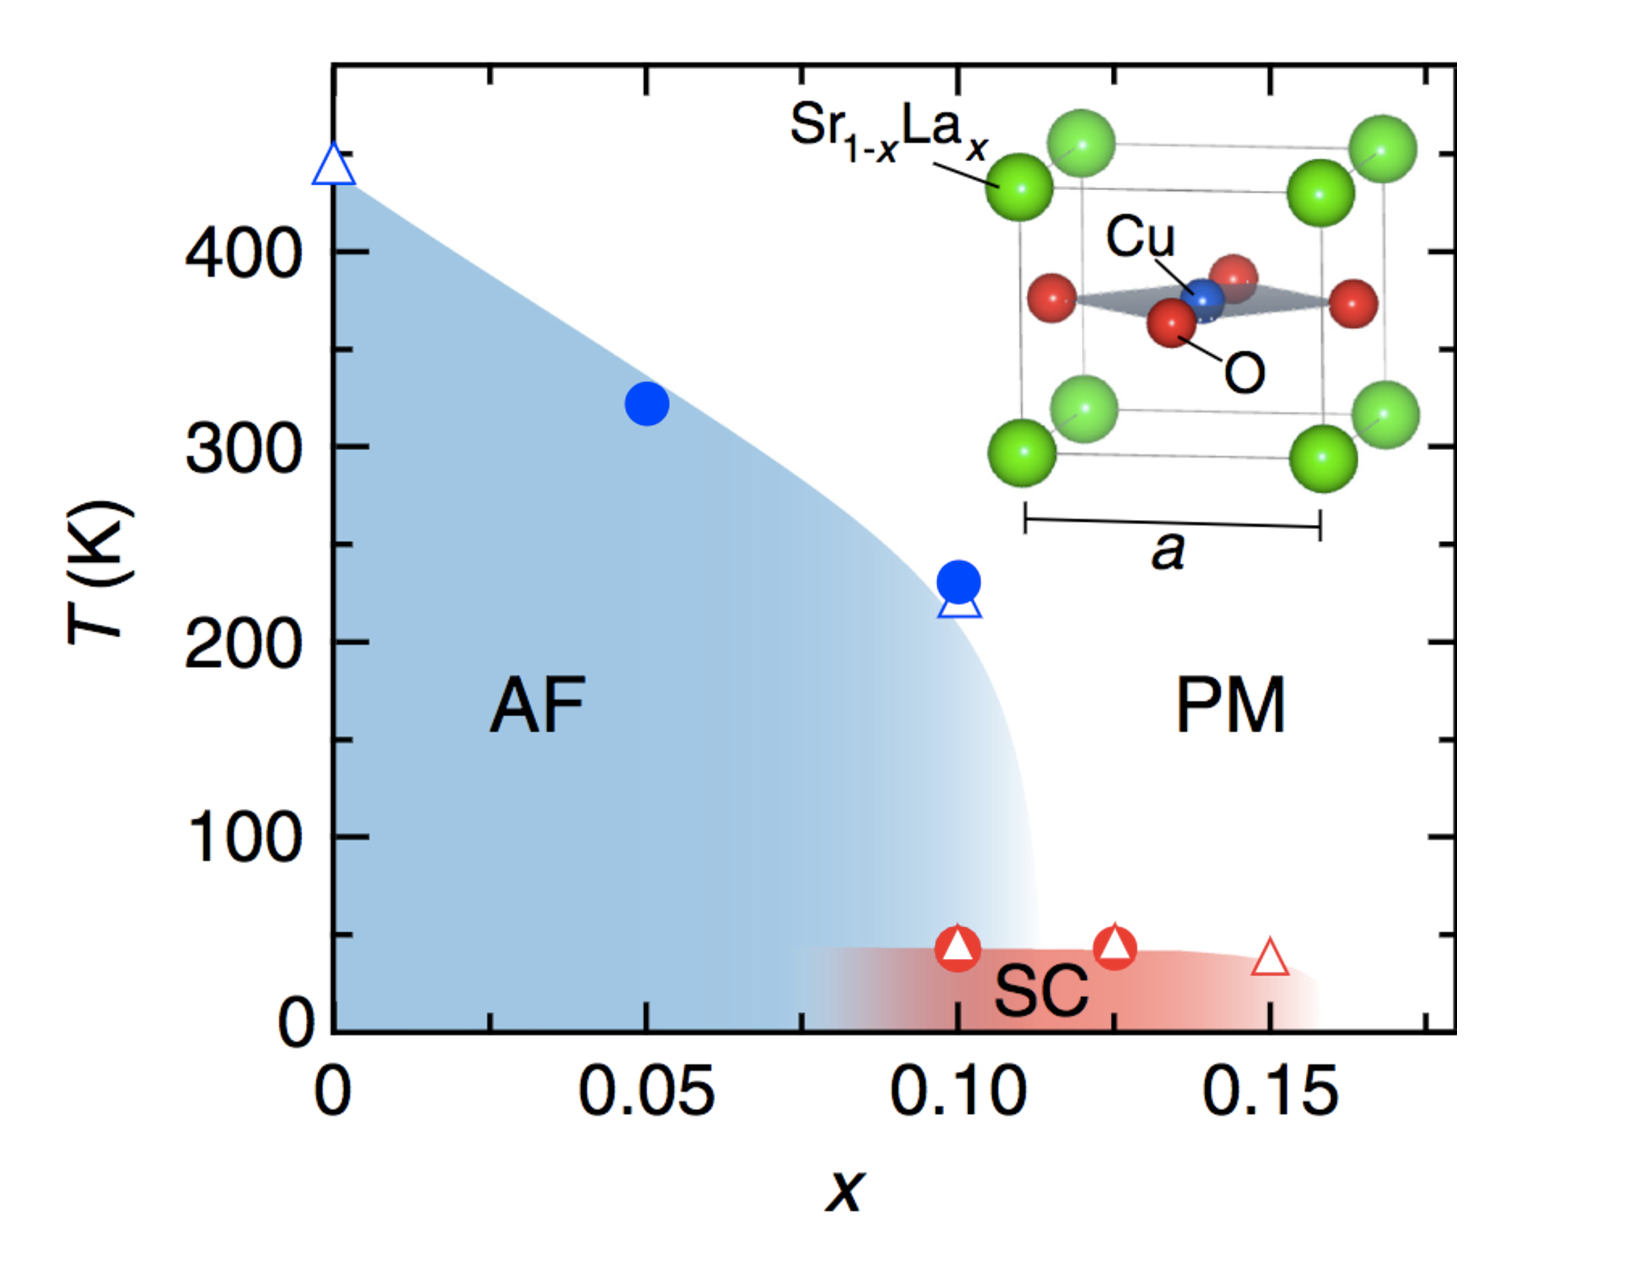
\includegraphics[width=0.6\textwidth]{Figures/I1-phase_diagram.pdf}
\caption{\label{fig1} Phase diagram of Sr$_{1-x}$La$_x$CuO$_2$ for various electron doping \textit{x} and temperature \textit{T}. Figure taken from [ref].}
\end{figure}

\begin{figure}[H]
\centering
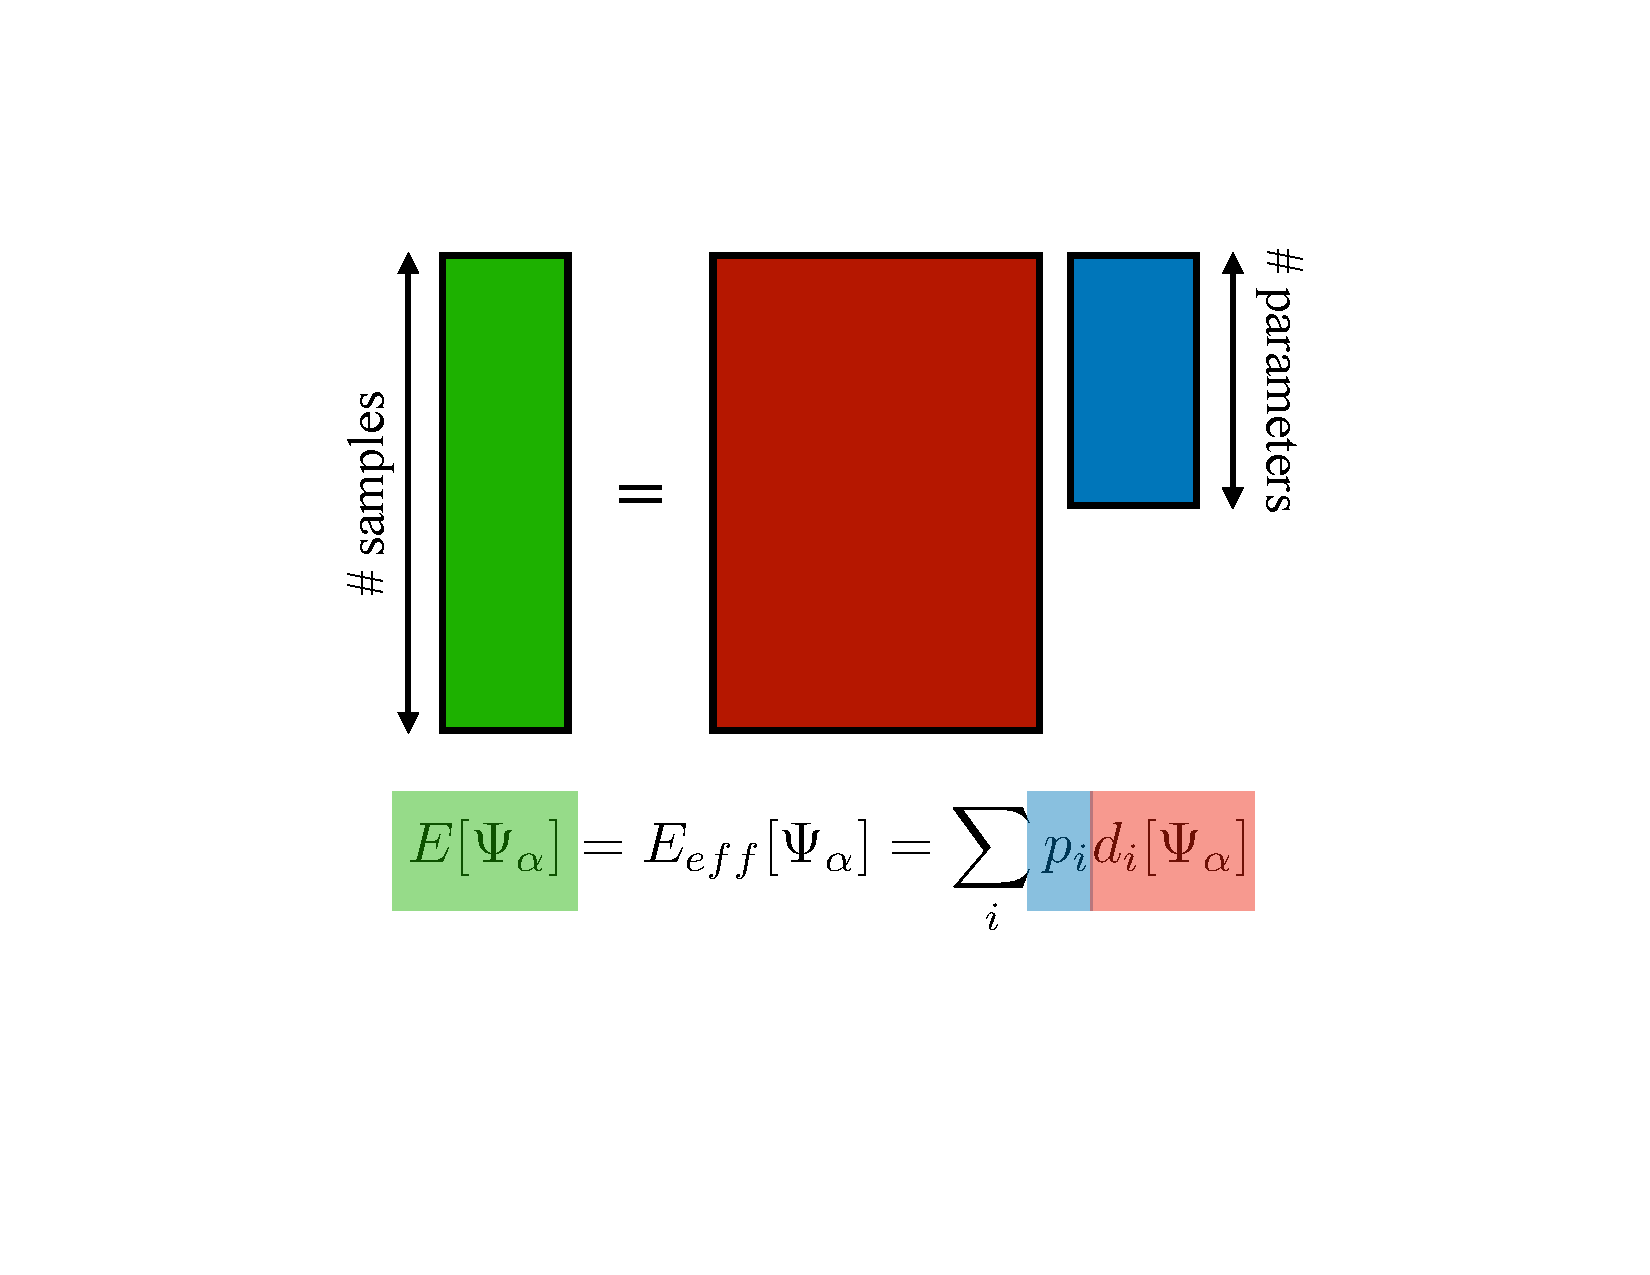
\includegraphics[width=0.9\textwidth]{Figures/I2-DMD_diagram.pdf}
\caption{\label{fig2} Schematic drawing of the the density matrix downfolding method, describing how the wave function samples, total energies, and descriptor values are mapped onto a linear regression problem.}
\end{figure}


\pagebreak

\section{Preliminary results and discussion}
\textit{The goal of the preliminary results is to indicate that I have the tools to actually complete the proposed research.}

\paragraph{NO determinants: Introduction} In order to become acquainted with our code  and QMC algorithms in general I worked on implementing and testing non-orthogonal orbital optimization in QWalk. 
\\
\textit{This paragraph should introduce the idea of non orthogonal orbital optimization.}

\paragraph{NO determinants: Work} The main work involved comparing the FN-DMC energies and single particle densities when using trial wave functions with and without non-orthogonal orbital optimization.
\\
\textit{This paragraph should include details about how we actually went about doing these calculations.}

\paragraph{NO determinants: Results and Discussion} We found that in addition to the improvements from orthogonal optimization, non-orthogonal orbital optimization yields improvements to the ground state FN-DMC energies and single particle properties.
\\
\textit{This paragraph should discuss the actual results from the calculations outlined above.}

\paragraph{SCO SCF: Introduction} To get a grasp on the relevant energy scales, model terms, and values for model parameters before trying the computationally expensive DMD with FN-DMC we attempted an \textit{ad hoc} fitting procedure using only DFT eigenvalues and total energies. 
\\
\textit{This paragraph should talk about the fitting procedure that we are planning on using.}

\paragraph{SCO SCF: Work} The task at hand was to generate low-energy states for the three different dopings x=0, 0.125, and 0.25 on a 2$\sqrt(2)$x2$\sqrt(2)$x1 unit cell and use them in our \textit{ad hoc} fitting procedure to generate an approximate effective model.
\\
\textit{This paragraph should talk about the procedural work of generating these low energy states and the mean field approximation for fitting. REMEMBER TO TALK ABOUT DROPPED STATES}

\paragraph{SCO SCF: Results and discussion} We find that a four parameter model with NN hopping, NNN hopping, AF Heisenberg exchange, and a FM NN Kondo term using only Cu 3d$_{x^2-y^2}$ orbitals can accurately describe the DFT band structures and total energies of low-energy states at T=0 and x=0, 0.125 and 0.25.
\\
\textit{This paragraph should talk about the results of the work from above.}

\paragraph{SCO DMD: Basis elements} Our first step into DMD with FN-DMC was the generation of appropriate basis elements for our effective model Hamiltonian which we handled, for all three dopings, using intrinsic atomic orbitals.
\\
\textit{This paragraph should talk about the IAO analysis that we have.}

\begin{figure}[H]
\centering
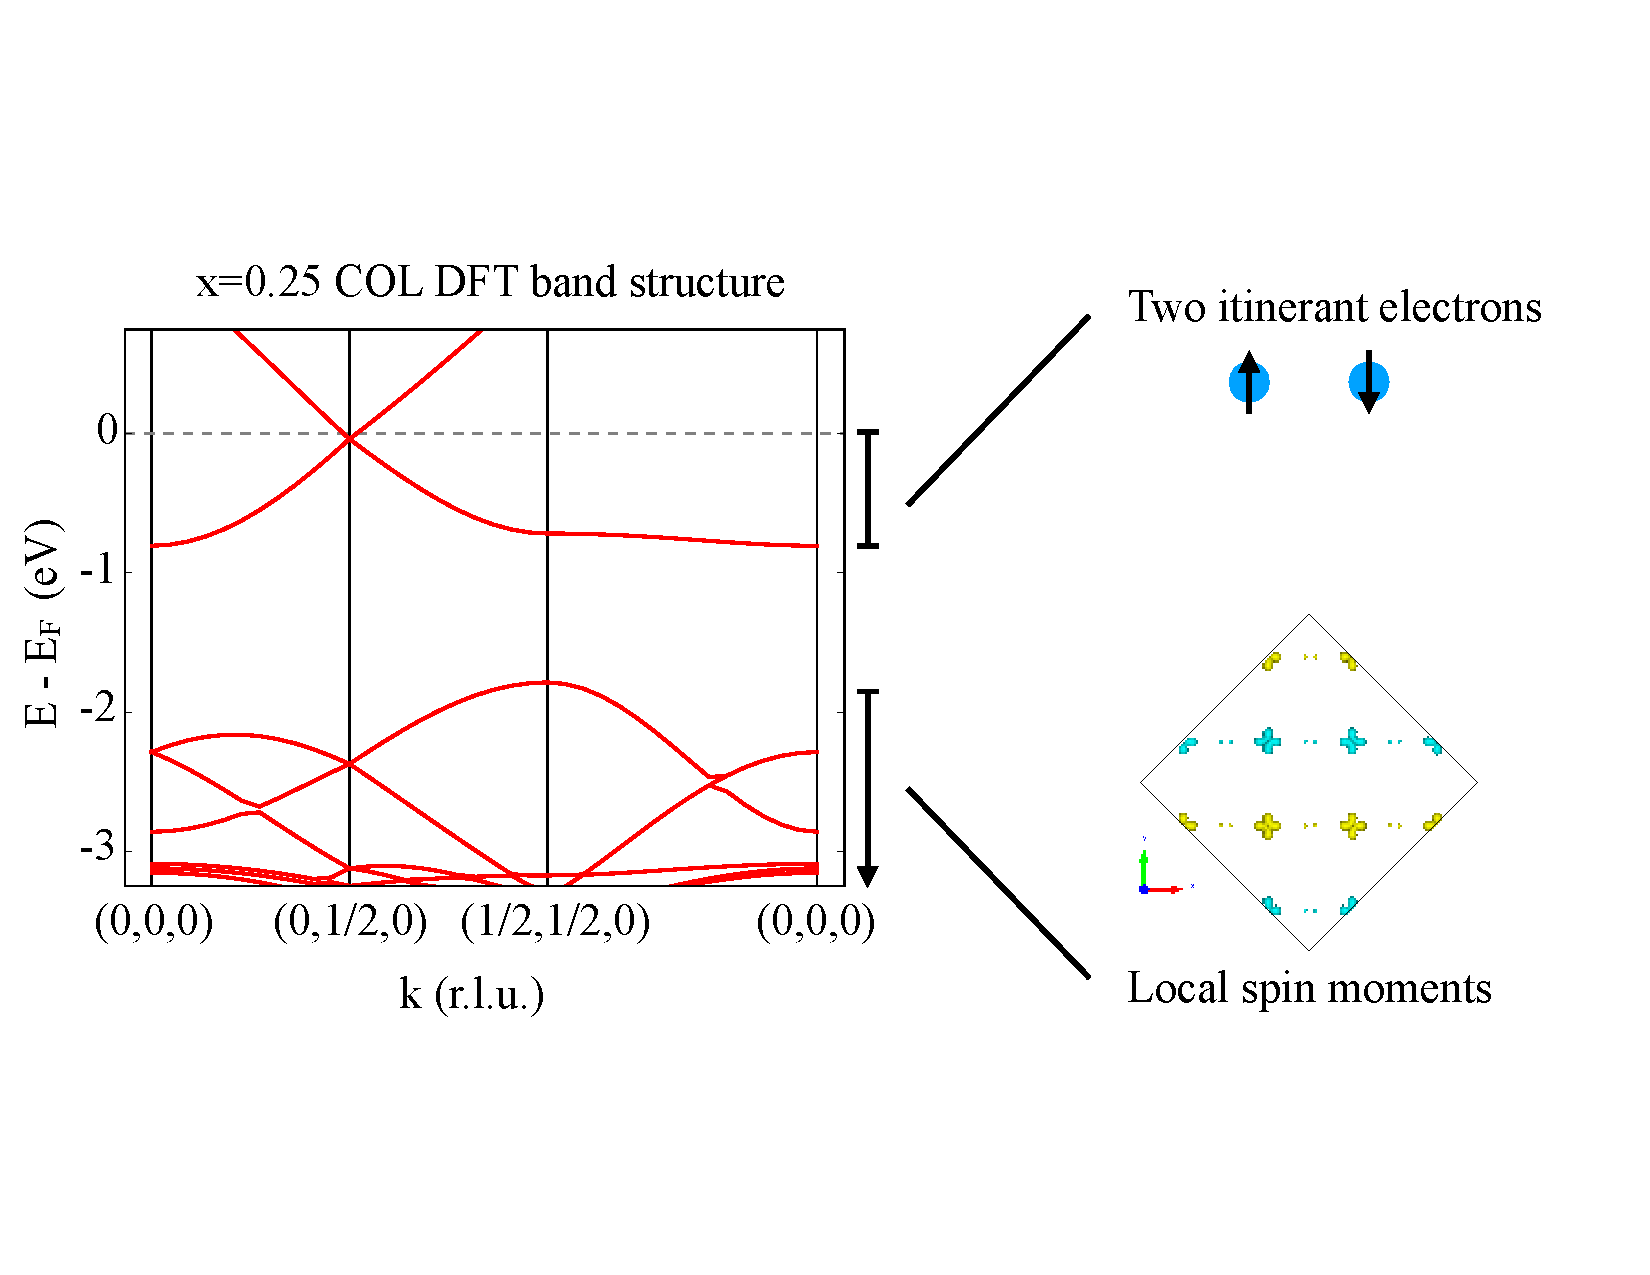
\includegraphics[width=0.6\textwidth]{Figures/R1-mean_field.pdf}
\caption{\label{fig3} Schematic diagram showing the method for mean-field approximation we used in our DFT model fitting calculations.}
\end{figure}

\begin{figure}[H]
\centering
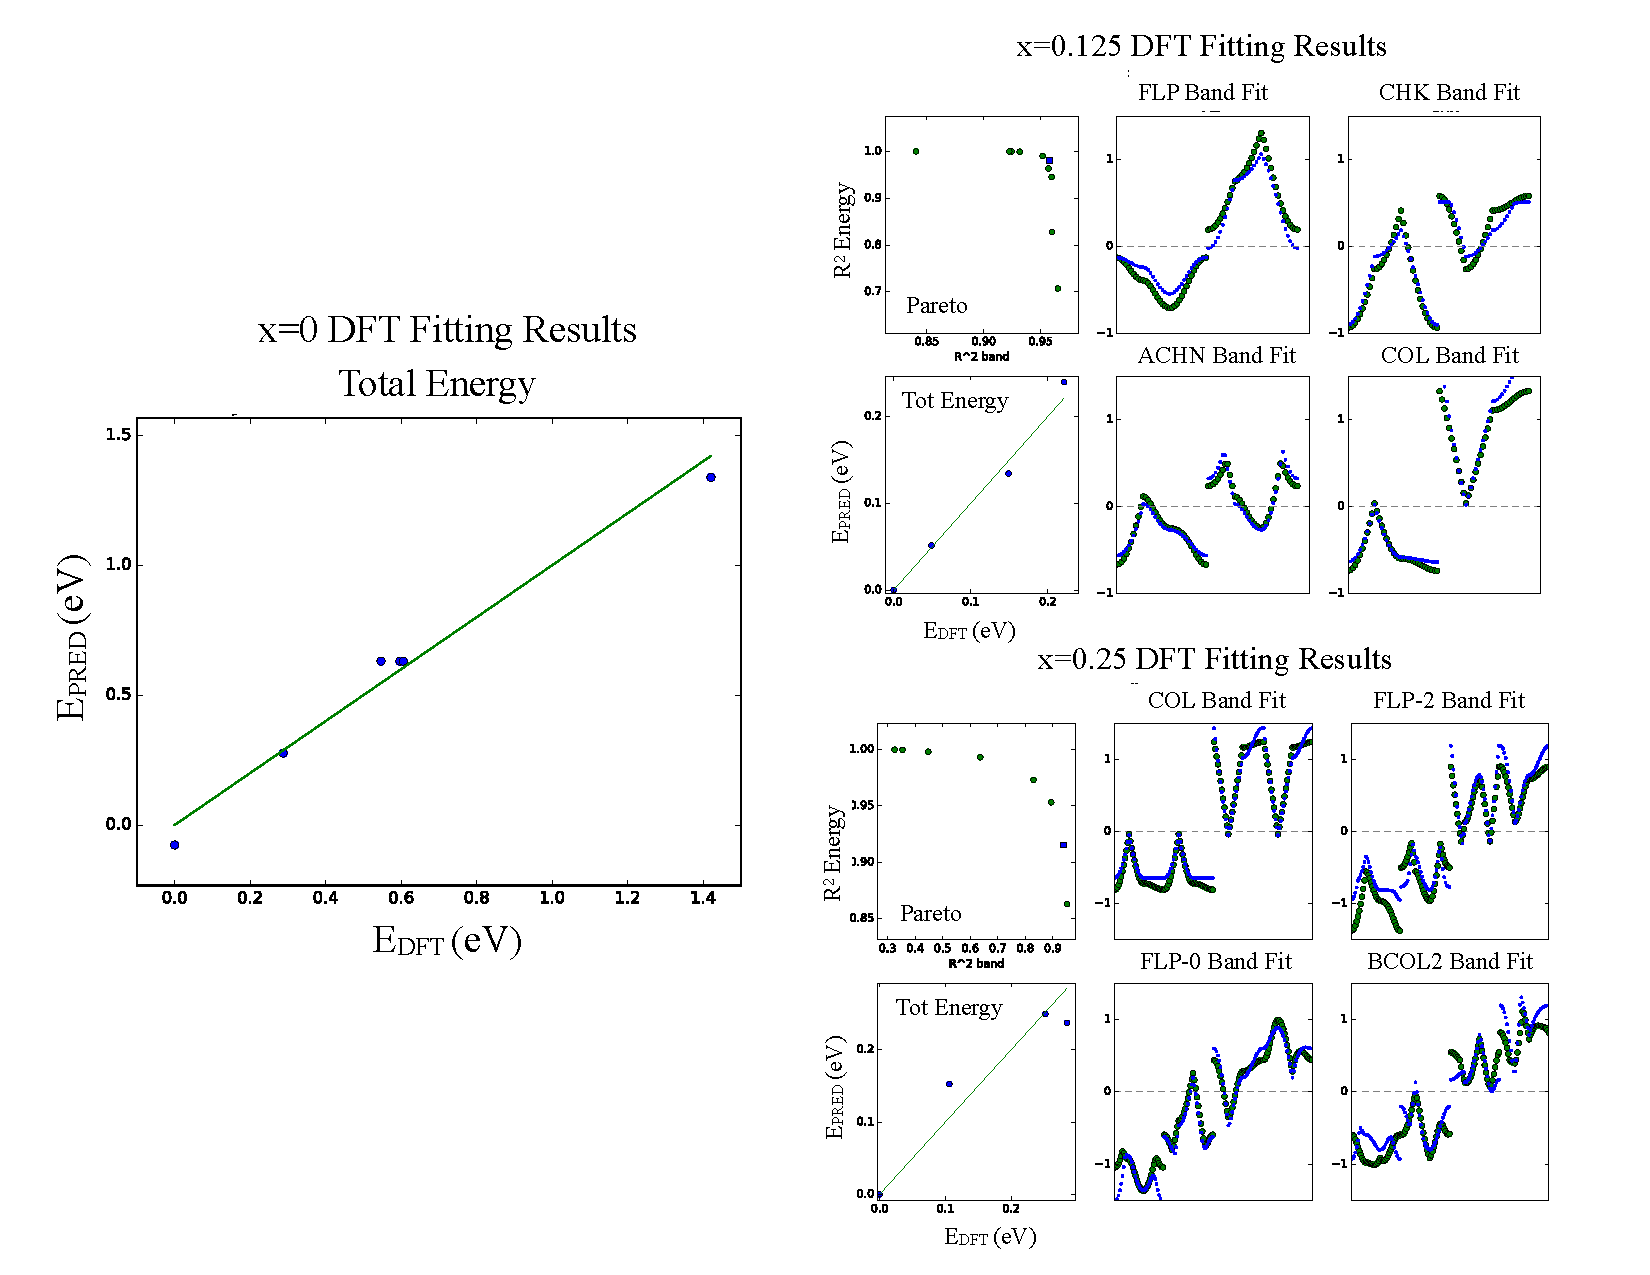
\includegraphics[width=0.9\textwidth]{Figures/R2-pareto.pdf}
\caption{\label{fig4} Results of the \textit{ad hoc} fitting procedure just using the DFT eigenvalues and total energies for three different dopings.}
\end{figure}

\begin{figure}[H]
\centering
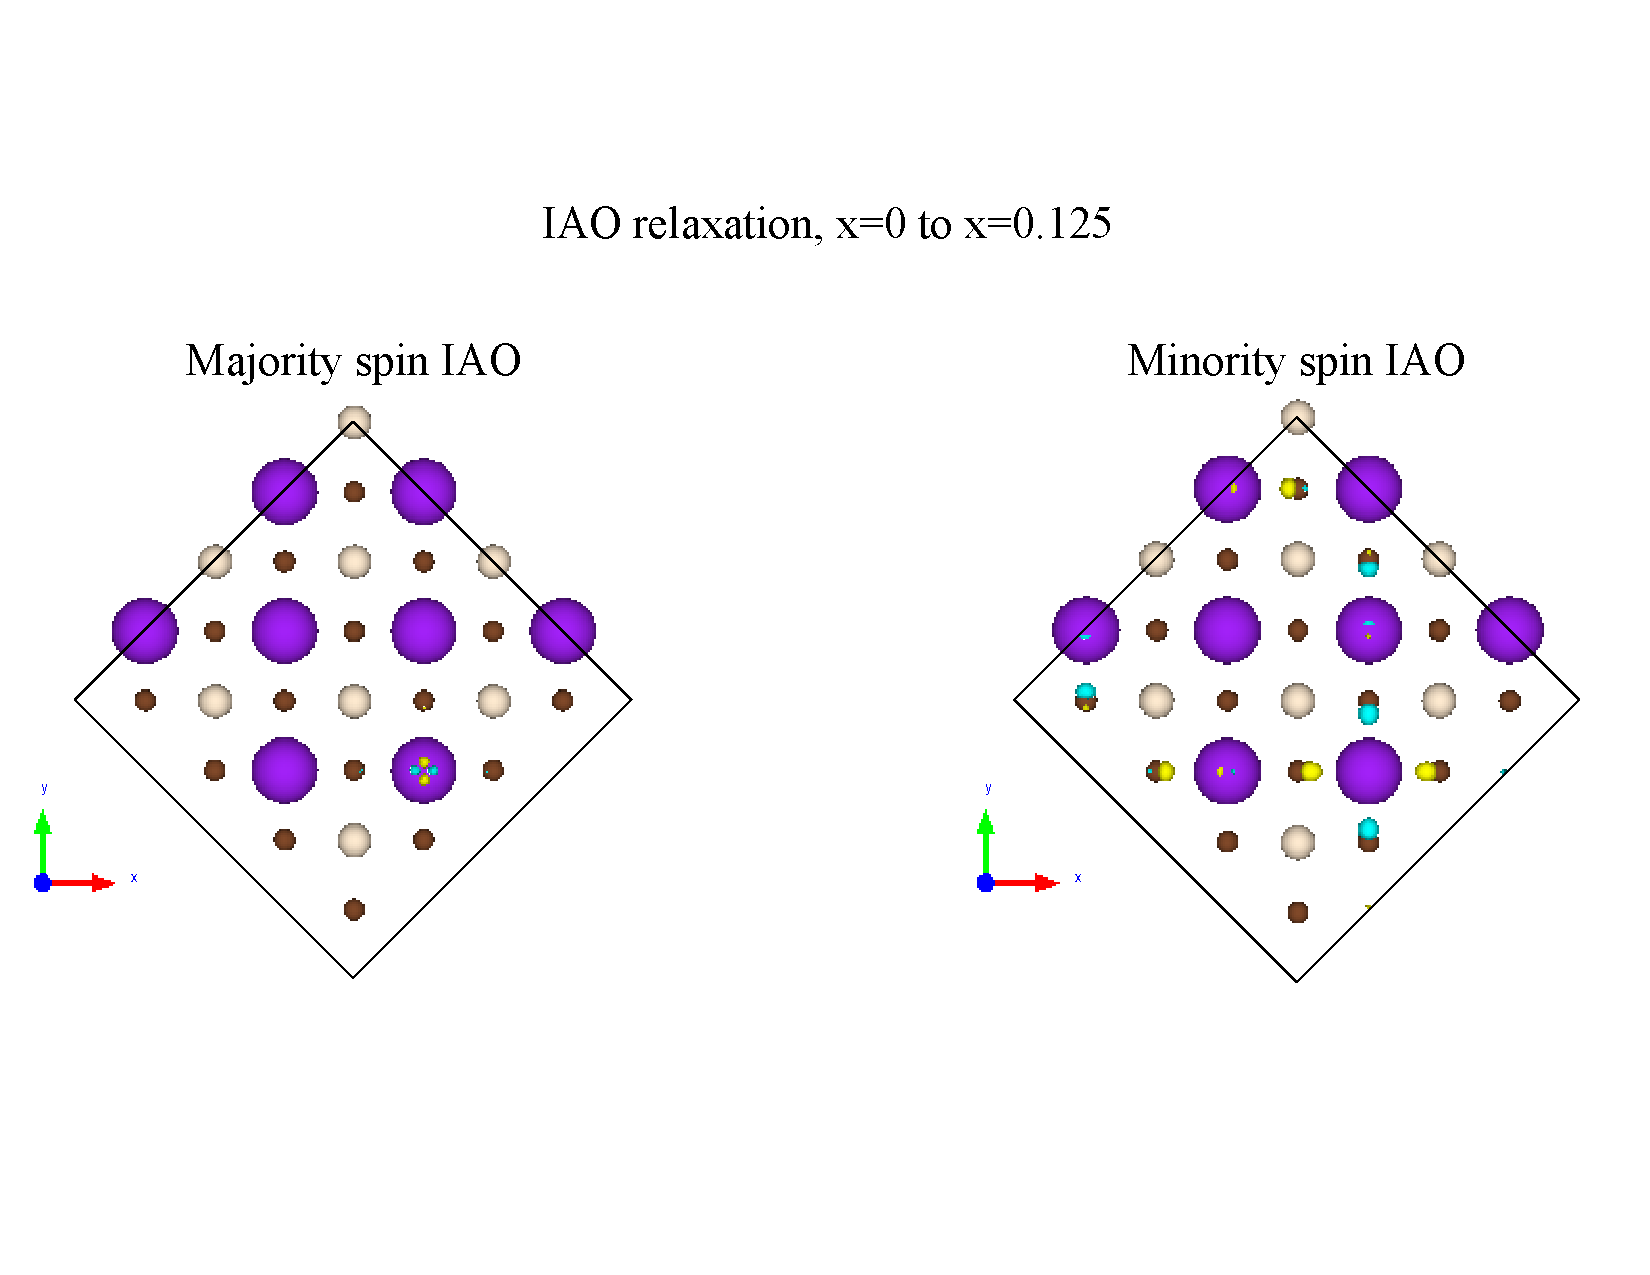
\includegraphics[width=0.9\textwidth]{Figures/R3-iao_basis.pdf}
\caption{\label{fig5} Relaxation of the IAOs for the spin majority and minority channel under doping for the eighth doped flip state. The majority spin IAO can be used as a basis for the fixed spin moments and the minority spin IAO for the itinerant electrons.}
\end{figure}
\pagebreak

\section{Proposed work}
\paragraph{SCO DMD: Low energy states} Low energy states for the x=0 system can be constructed by using DFT states with different spin textures multiplied by a 3-body Jastrow factor as trial wave functions in FN-DMC.
\\
\textit{This paragraph should talk about low energy states for x=0 and the DMD procedure (no parameter derivatives).}

\paragraph{SCO DMD: Low energy states} For the doped systems, low energy states will be constructed using multi-determinant expansions composed of low energy DFT states and singly excited determinants multiplied by a 3-body Jastrow factor as trial wave functions in FN-DMC.
\\
\textit{This paragraph should talk about the linear combination states and parameter derivatives.}

\paragraph{SCO: Band structure} In addition to using them in the DMD procedure, we will use these low energy multi-determinant expansions to generate effective band structures for the doped states.
\\
\textit{This paragraph should talk about the independent project of using parameter derivatives for band structure on large systems.}

\paragraph{SCO DMD: Descriptors} After calculating the RDMs on our IAO basis using FN-DMC, the relevant descriptors in our model can be initially restricted through symmetry considerations.
\\
\textit{This paragraph should talk about symmetry restriction of descriptors.}

\paragraph{SCO DMD: Descriptors} Further restriction of relevant descriptors will be accomplished by using a greedy selection algorithm.
\\
\textit{Talk about the greedy algorithm.}

\paragraph{SCO DMD:  FSE and K-points} QMC calculations on solids are accompanied by finite size effects which we will deal with, if necessary, using either a supercell extrapolation, k-point (twist) averaging, or both.
\\
\textit{Talk about how we would be able to diagnose whether FSE is important, then talk about how each of these methods work.}
 
 \paragraph{SCO DMD: Reach goal} A longer term goal is to use the DMD method to generate a single low-energy model that can accurately describe the low-energy properties of both superconducting SCO and an isostructural non-super conducting nickelate.
 \\
 \textit{This should talk about the goal of showing that DMD is actually accurate in its predictions, and is an interesting scientific problem not just a calculation we did.}

\begin{figure}[H]
\centering
%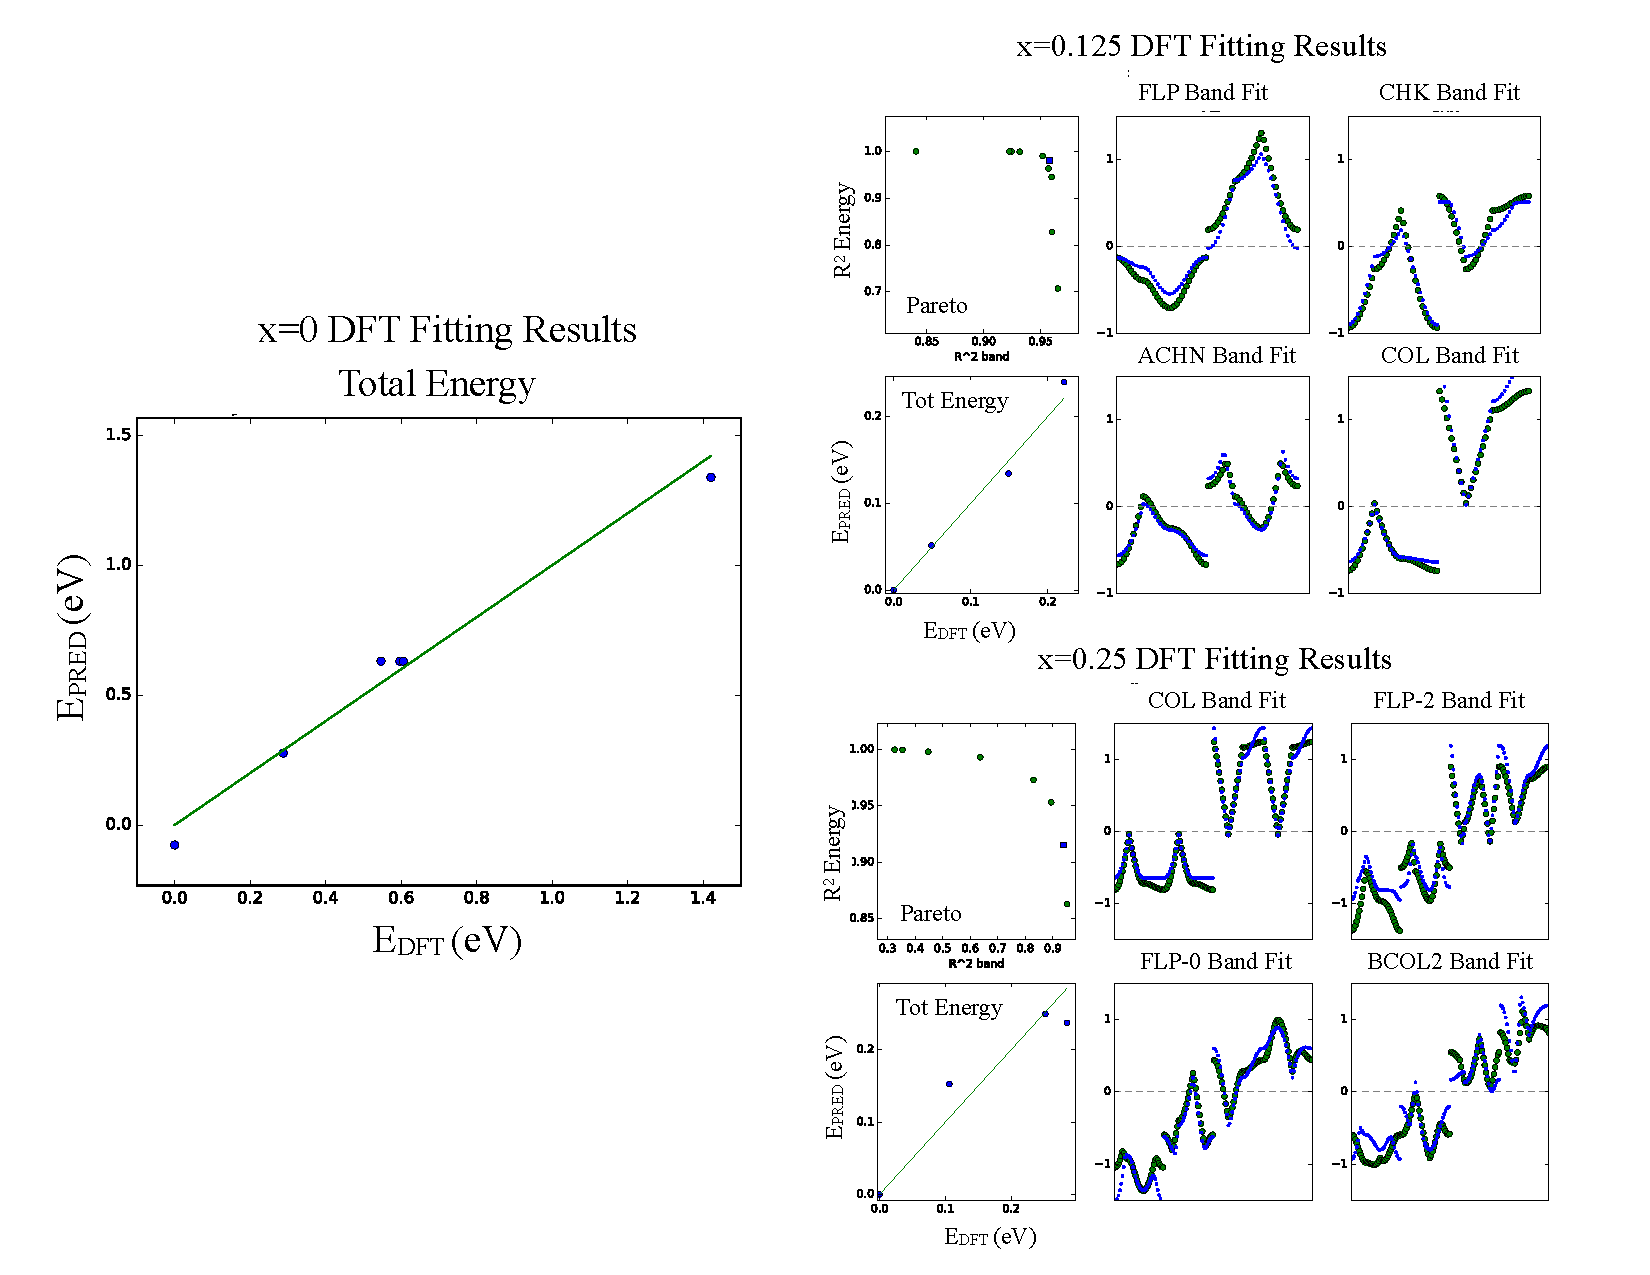
\includegraphics[width=0.9\textwidth]{Figures/R2-pareto.pdf}
\caption{\label{fig6} Results for greedy algorithm procedure for choosing descriptors showing the decrease in $R^2$ as more descriptors are added for the FeSe molecule [ref].}
\end{figure}

\begin{figure}[H]
\centering
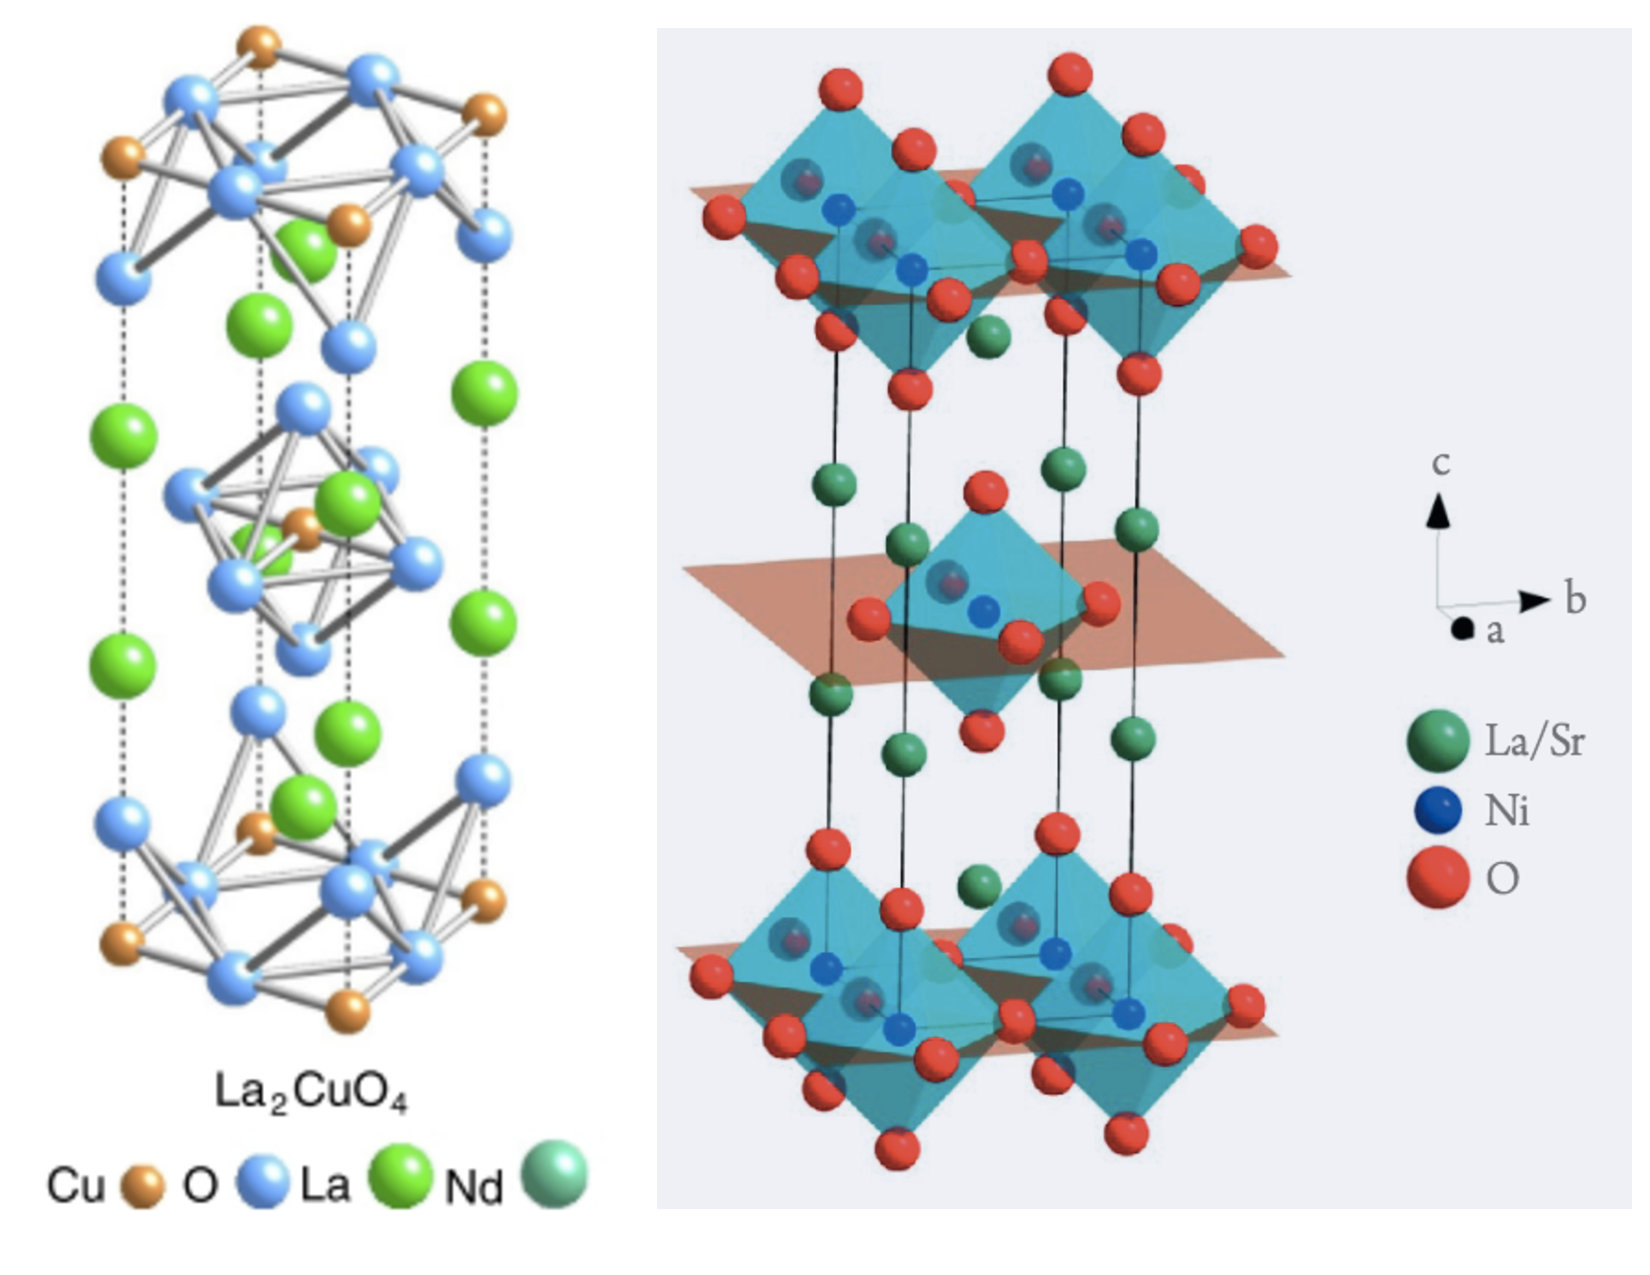
\includegraphics[width=0.9\textwidth]{Figures/P2-Ni_Cu.pdf}
\caption{\label{fig7} The primitive unit cells of the isostructural materials LNCO [ref] and LSCO [ref], the prior which is not super conducting all the way to temperatures of 30mK [ref].}
\end{figure}
\pagebreak

\section{Conclusion and Summary}
\paragraph{SCO DMD} We propose that a DMD method using \textit{ab initio} QMC calculations can generate an effective model which can describe the low-energy properties of the electron doped cuprate SCO with a level of accuracy previously unattainable.

\paragraph{SCO Reach goal} We hope to extend our model fitting calculation to gain insight into why materials like nickelates, which are isostructural to the cuprates, do not superconduct. 

\end{document}